% document settings
\documentclass[a4paper, openany]{book}
\usepackage{amsmath, amsthm, amssymb, graphicx}
\usepackage{geometry,fontspec, xeCJK, indentfirst}

% document layout and style settings
\usepackage[bookmarks=true, colorlinks, citecolor=blue, linkcolor=black]{hyperref}
\usepackage{amsmath, cleveref, caption, subcaption}
\usepackage[T1]{fontenc}
\usepackage{textcomp}
\geometry{a4paper, scale = 0.8}
\setmainfont{Noto Serif}
\setsansfont{Noto Sans}
\setmonofont{Noto Sans Mono}
%\setCJKmainfont{Noto Serif SC}
%\setCJKsansfont{Noto Sans SC}
\setlength{\parindent}{2em}
\captionsetup{format = hang, font = small, labelfont = bf, labelsep = quad}

% metadata
\title{Note for Computational Analysis}
\author{Zhen-Lin Huo, Robin Song}
\date{\today}

% document content
\begin{document}

\maketitle
\frontmatter
\tableofcontents

% main content starts from here
\mainmatter

\chapter{Introduction}

This note is for course \textbf{BARC0030 Computational Analysis} of Architectural Computation MSc., Bartlett School of Architecture, University College London. This course is taught by Prof. \textbf{Sean Hanna}.

In this course, you will learn some basic knowledge for design with computational methods, together with an introduction to machine learning.

This note bases on my note for this course, and with the help of my friend \textbf{Robin Song}. Our goal is to help anyone who has interest in \textbf{Space Syntax}, \textbf{Computational Design}, and \textbf{Machine Learning} to briefly understand the basic knowledge, principle, and philosophy for corresponding cources.

Finally, hope you can enjoy!

Zhen-Lin Huo

2025-05-19

\chapter{Information Theory \& Formal System}

To start with, let's talk about the most basic concept about computation: information.

Information is everywhere, even when there is no computer: when you ask your friend `Do you want to hang out and have McDonald's with me?', you already send a piece of information to your friend.

\begin{quotation}
The only way to rectify our reasoning is to make them as tangible as those of the Mathematicians, so that we can find our error at a glance, and when there are disputes among persons, we can simply say: Let us calculate (calculemus), without further ado, to see who is right.

\hfill ---Leibniz, The Art of Discovery (1685)
\end{quotation}

\section{Information}

\subsection{Entropy 熵}

Entropy of X is the amount of uncertainty in X

\emph{associated with X}

entropy = information

Quantify:

\begin{itemize}
  \item \(S = \mathit{k} \log W\) (Boltzmann)
  \item \(H ( X ) = -\sum_{\mathit{x}\in X}^{} p ( \mathit{x} ) \log p ( \mathit{x} )\)
\end{itemize}

\subsection{Shannon-Fano Coding (Fano's
Method)}

In a piece of given information (e.g. a sentence):

\begin{enumerate}
  \item Calculate the frequency of each character
  \item Divide the characters into two groups (0 and 1) based on their
  frequencies
  \begin{itemize}
    \item make each group has approximately 50\% of the total frequency
  \end{itemize}
  \item Repeat the process to that 2 groups, until each group has only one
  character
\end{enumerate}

Actual entropy of given message:

\[H ( X ) = -\sum_{\mathit{x}\in X}^{} p ( \mathit{x} ) \log p ( \mathit{x} )\]

Mean word length:

\[E\left [ \mathit{I} ( \mathit{x} )  \right ] =  \sum_{\mathit{x}\in X}^{} p ( \mathit{x} ) Level\]

\subsection{Communication}

\textbf{Mutual Information}

\[\mathit{I} ( \mathit{X}; \mathit{Y} ) = \mathit{H} ( \mathit{Y} ) - \mathit{H} ( \mathit{Y} \mid \mathit{X} )\]

\textbf{Channel Capacity}

\[\max_{\mathit{f}} \mathit{I} ( \mathit{X}; \mathit{Y} )\]

Channel capacity is determined by:

\begin{itemize}
  \item Message coding
  \item Noise
\end{itemize}

\section{Formal System}

Formal system is a set of rules controlling how things runs. In other word, a formal system has following characteristics:

\begin{itemize}
  \item Have Syntax
  \item Not Semantics (no meanings)
\end{itemize}

It is believed that if something can be converted into a formal system, it would be totally logistic, thus can be `understanded' and processed by a computer.

\subsection{Formalising Language}

So, here comes our greatest example for formal system: formalising language.

\subsubsection{Finite State (Markov) Grammar}
\label{sec:markov-grammar}

One of the most simple way to construct a sentence is to use Markov Model (\textbf{\cref{sec:markov-model}}): a system that changes state according to a probability distribution based on previous states.

Treat each word as a state, then a sentence can be constructed by a Markov Process.

\emph{1\textsuperscript{st} order}

\begin{figure}[htbp]
  \centering

  \parbox[t]{0.29\textwidth}{The man comes

    The men come}
  \begin{subfigure}{0.39\textwidth}
    \raggedright
    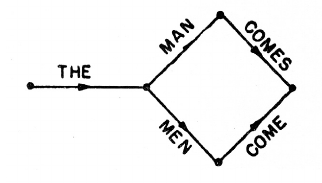
\includegraphics[width=0.5\textwidth]{assets/MarkovGrammar1.png}
  \end{subfigure}
\end{figure}

or

\begin{figure}[htbp]
  \centering
  \parbox[t]{0.29\textwidth}{The old man comes

    The old men come}
  \begin{subfigure}{0.39\textwidth}
    \raggedright
    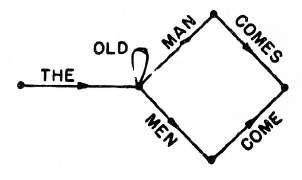
\includegraphics[width=0.5\textwidth]{assets/MarkovGrammar2.png}
  \end{subfigure}
\end{figure}

No memory $\rightarrow$ Cannot solve complex order

\emph{n\textsuperscript{th} order}

\begin{quotation}
  The old man I met last week comes

  The old men I met last week come
\end{quotation}

\subsubsection{Chomsky (1957): Grammar as Recursive
Rules}

\begin{itemize}
  \item S $\rightarrow$ NP + VP
  \item NP $\rightarrow$ N + auxP
\end{itemize}

\begin{figure}[htbp]
  \centering
  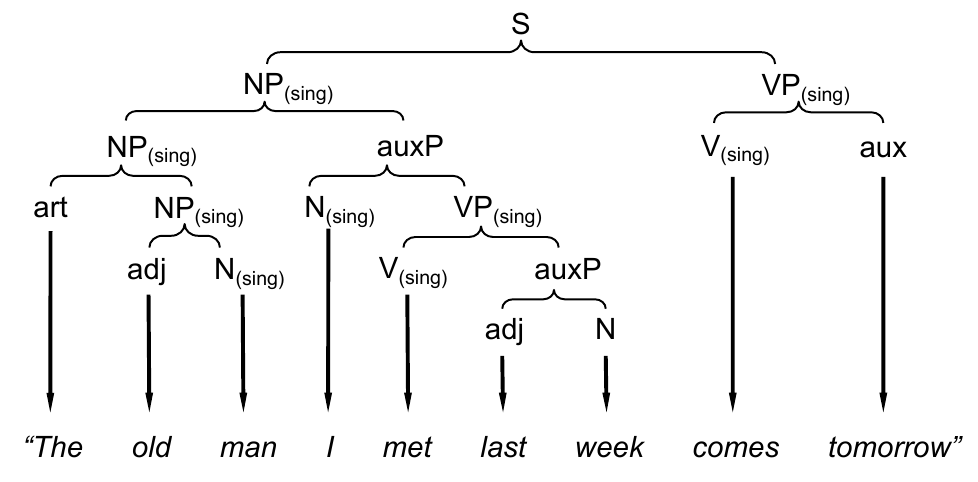
\includegraphics[width=0.8\textwidth]{assets/GrammarAsRecursiveRules1.png}
\end{figure}

\subsubsection{Characteristica Universalis}

Firstly proposed by Gottfried Leibniz in 17\textsuperscript{th} century.

An idea for a /textbf{universal symbolic language} --- especially in /textbf{logic, mathematics, science, and philosophy}. Leibniz believed that if we could reduce reasoning to a kind of calculation using symbols, then disagreements could be resolved by computation, like solving an equation.

\paragraph{Construction of \textit{Characteristica Universalis}}

\begin{itemize}
  \item \textbf{Symbols for Concepts}: For every basic idea of concept
  \item \textbf{Combinatorial Rules}: Complex ideas would be built by combining simpler ones, using logical and mathematical rules—similar to how algebra or programming languages work.
  \item \textbf{Logical Structure}: Tightly connected to \textbf{formal logic}, so reasoning could be done mechanically just like a machine, following steps.
  \item \textbf{Inspired by Mathematics}: As precise and unambiguous as mathematics, so that can avoid the vagueness of natural languages.
\end{itemize}

\subsubsection{David Hilbert (1900): Attempt to Complete It}

23 problems (to be resolved by 20\textsuperscript{th} century mathematics)

\subsection{Computer Cognition}

Since there exists a method to construct sentence, scientists also tried to discuss whether a computer can `understand' information, and is it important for dealing with information.

\subsubsection{Turing Test}

Recognising intelligence: how to evaluate whether a computer has intelligence?

Alan Turing (1949), the imitation game:

\begin{itemize}
  \item A man (\textbf{A}) in a room, communicating with another man (\textbf{C}) with text
  \item A computer (\textbf{B}) in the same room, communicating with (\textbf{C})
  \item If \textbf{C} cannot distinguish \textbf{B} as a computer or a human, then \textbf{B} is intelligent
\end{itemize}

\subsubsection{ELIZA (1665)}

A Computer Programme for the Study of Natural Language Communication between Man and Machine

\begin{flushright}
  ---Joseph Weizenbaum, 1966
\end{flushright}

\begin{itemize}
  \item Pick some key words from human reply, and ask questions about these words.
  \item `Simulating intelligence'
\end{itemize}

\subsubsection{Searle's `Chinese Room' (1980)}

Extension of Turing Test:

\begin{itemize}
  \item Searle is the one in the room, and he doesn't understand Chinese
  \item a series of instructions are given to Searle, telling him what to reply when seeing different messages.
  \item Outer people cannot tell whether Searle himself understand  Chinese or not
\end{itemize}

\textbf{Dualism in The Mind}

The Chinese Room argument split language into \textbf{syntax} (rules in the instructions) and \textbf{semantics} (understanding the meaning of the words in mind).

It suppose: A symbolic (mental) level must be essentially arbitrary and meaningless and it maps easily onto the real world.

\subsection{Limitation of Formal System}

Is a formal system perfect to represent information and deal with all kinds of problems?

\subsubsection{Gödel's Incompleteness Theorems (1931)}

\begin{quotation}
  For every $\omega$-consistent recursive class $\kappa$ of formulas, there are recursive class signs $\mathsf{r}$ such that neither $\forall \mathsf{vr}$ nor $\neg \forall \mathsf{vr}$ is in $\kappa$.
\end{quotation}

This means, in a consistent formal system, there are always some true statements that cannot be proved within that system. 

\begin{quotation}
  e.g.
  \begin{enumerate}
    \item Sentence \# 2 is true.
    \item Sentence \# 1 is false.
  \end{enumerate}

  And\dots

  There exists no proof of this statement.
\end{quotation}

\subsubsection{About Formal System}

Gödel described a way to number a formal system. e.g.

\hspace*{\fill}

\begin{tabular}{ccl}
  Sign & Gödel \# & Meaning \\
  \hline
  $\neg$ & 1 & not \\
  $\lor$ & 2 & or \\
  $\supset$ & 3 & if \dots then \\
  $\exists$ & 4 & there exists \\
  $=$ & 5 & equals \\
  $0$ & 6 & zero \\
  $s$ & 7 & immediate successor \\
  $($ & 8 & \\
  $)$ & 9 & \\
  $,$ & 10 & \\
  $+$ & 11 & plus \\
  $\times$ & 12 & times \\
\end{tabular}
\qquad
\begin{tabular}{ccc}
  Sign & Gödel \# & Possible Substitution \\
  \hline
  $x$ & 13 & 0 \\
  $y$ & 14 & s0 \\
  $z$ & 15 & y \\
  $p$ & $13^2$ & $0 = 0$ \\
  $q$ & $17^2$ & $( \exists x ) ( x = sy )$ \\
  $r$ & $19^2$ & $p \supset q$ \\
  $P$ & $13^3$ & $x = sy$ \\
  $Q$ & $17^3$ & $\neg ( x = ss0 \times y )$ \\
  $R$ & $19^3$ & $( \exists z ) ( x = y + sz )$
\end{tabular}

\hspace*{\fill}

\hspace*{\fill}

Then a formal system can be numbered like below:

$$e.g. \  ( \exists x ) ( x = sy )$$

\begin{figure}[htbp]
  \centering
  \includegraphics[width=15em]{assets/GödelNumber1.png}
\end{figure}

Gödel number of it can be calculated:
$$m = 2^8 \times 3^4 \times 5^{13} \times 7^9 \times 11^8 \times 13^{13} \times 17^5 \times 17^5 \times 19^7 \times 23^{17} \times 29^9$$

Gödel number for sequence of formulas:
$$( \exists x ) ( x = sy ) \  \rightarrow \  m$$
$$( \exists x ) ( x = s0 ) \  \rightarrow \  n$$
$$\mathsf{sequence} \  k = 2^m \times 3^n$$

So that any expression (e.g. formula, proof, etc.) as a Gödel number.

\textbf{\textit{Question: How to understand the relationship between the Gödel number and whether it can be proved?}}

\dots And finally, we can see, in a consistent formal system, there are always some true statements that cannot be proved within that system.

\section{Non-Formal Alternatives}

To conclude, Leibniz proposed the ideal of formalising and formal language, and Gödel proved that the formal systems are limited.

\begin{quotation}
  Since man at least adapts (a truism, for any large dynamic system does so) there is no genuine `channel capacity' in Shannon's (1949) sense. For the load imposed by an input may depend upon all of the inputs received up to the moment in question. Or put commonsensically, as it may be if the subject is assumed to learn input/output relations, a once difficut task will become less difficult as the task relation is learned.

  \hfill ---Pask G, \textit{Communication Cognition and Learning}, 1975
\end{quotation}

The language may not be formal, because they showed great ambiguity.

\subsection{Grammatical Structure}\label{sec:grammatic-structure}

Think back to Markov Chain and Finite State Machine, we can subdivide the state of a finite state machine, so they can do better than the previous version (\textbf{\cref{sec:markov-grammar}}).

\begin{figure}[htbp]
  \centering
  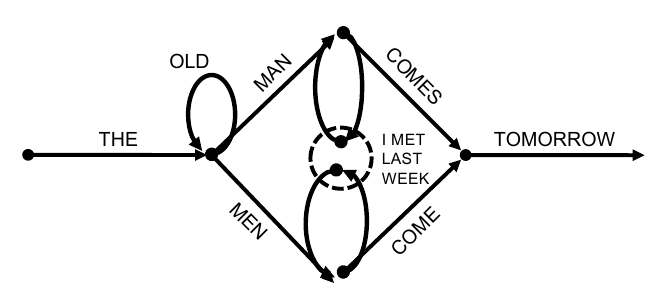
\includegraphics[width=20em]{assets/GrammaticStructure1.png}
\end{figure}

\subsection{Predicting Grammatical Structure (Jeffrey Elman): A Dynamical System}

\subsubsection{Neural Network}

The previous mentioned Markov process (\textbf{\cref{sec:grammatic-structure}}) can be coded into a neural network:

\begin{quote}
  input unit(s) --- recurrent layer --- output unit(s)
\end{quote}

The recurrent layer can capture changes (word sequence) over time.

After training, this network is able to predict what type of word will come next in a sentence.

In this network, \textbf{syntax} and \textbf{semantics} are in the same space.

\subsubsection{Words \& Sentences in High Dimensional Space}

\paragraph{Convert Words into Vectors}

In this neural network, each word activates neurons in the hidden layer differently, which can be mapped as vectors in a high dimensional space (state space).

A single word will correspond to a series of points in the state space.

\paragraph{Sentence in State Space}

As a sentence is a sequence of words, constructing a sentence is just connecting different points / vectors in the state space.

The same word with different grammatical context will have similar but not same route in the state space.

\chapter{Space Syntax}

\chapter{System Dynamics: Emergence, Divergence, Convergence}

\chapter{Machine Learning Introduction}

\section{Abstract Model of Computer}

\subsection{Finite State Machine}

A theoretical computing machine

Alan Truing

\begin{itemize}
  \item The machine can be in one of a finite number of states
  \item Can change (academically, \emph{transit}) from one state to another in
  response to some inputs
\end{itemize}

\subsection{Turing Machine}

Alan Turing (1936)

\begin{itemize}
  \item A tape
  \begin{itemize}
    \item Has infinite length
    \item Is divided into cells
    \item Is blank, or contain a symbol
  \end{itemize}
  \item The head
  \begin{itemize}
    \item Can read/write/erase
    \item Can move left/right
  \end{itemize}
  \item State Register
  \begin{itemize}
    \item Machine can be one a number of states
  \end{itemize}
  \item Transition Table
  \begin{itemize}
    \item Erase/Write a symbol
    \item Move the head (L/R)
    \item Change machine state
  \end{itemize}
\end{itemize}

\subsection{Universal Turing Machine}

Universal Turing Machine~simulates a Turing Machine. It contains a
Turing Machine description as input along with an input string, runs the
Turing Machine on the input and returns a result.

Turning Machine + Encoded Type (Programme) = Universal Turing Machine

\subsection{Markov Model}
\label{sec:markov-model}

\begin{itemize}
  \item have a finite set of states
  \item different states (or group of states) have different probabilities to
  turn into other states (or itself)
\end{itemize}

If add memory into the Markov Model, we can get a second-order Markov
Model (dependent on (t-1) and (t))

The system will look different depending on how the states are defined.

\end{document}
